\documentclass[a4paper]{book}
\usepackage{a4wide}
\usepackage{makeidx}
\usepackage{graphicx}
\usepackage{multicol}
\usepackage{float}
\usepackage{listings}
\usepackage{color}
\usepackage{textcomp}
\usepackage{alltt}
\usepackage{times}
\usepackage{ifpdf}
\ifpdf
\usepackage[pdftex,
            pagebackref=true,
            colorlinks=true,
            linkcolor=blue,
            unicode
           ]{hyperref}
\else
\usepackage[ps2pdf,
            pagebackref=true,
            colorlinks=true,
            linkcolor=blue,
            unicode
           ]{hyperref}
\usepackage{pspicture}
\fi
\usepackage[utf8]{inputenc}
\usepackage{doxygen}
\lstset{language=C++,inputencoding=utf8,basicstyle=\footnotesize,breaklines=true,breakatwhitespace=true,tabsize=8,numbers=left }
\makeindex
\setcounter{tocdepth}{3}
\renewcommand{\footrulewidth}{0.4pt}
\begin{document}
\hypersetup{pageanchor=false}
\begin{titlepage}
\vspace*{7cm}
\begin{center}
{\Large Reference Manual}\\
\vspace*{1cm}
{\large Generated by Doxygen 1.6.3}\\
\vspace*{0.5cm}
{\small Thu Mar 10 19:13:29 2011}\\
\end{center}
\end{titlepage}
\clearemptydoublepage
\pagenumbering{roman}
\tableofcontents
\clearemptydoublepage
\pagenumbering{arabic}
\hypersetup{pageanchor=true}
\chapter{Class Index}
\section{Class Hierarchy}
This inheritance list is sorted roughly, but not completely, alphabetically:\begin{DoxyCompactList}
\item \contentsline{section}{VAbstractCalibrator}{\pageref{classVAbstractCalibrator}}{}
\begin{DoxyCompactList}
\item \contentsline{section}{VMonoCalibrator}{\pageref{classVMonoCalibrator}}{}
\item \contentsline{section}{VStereoCalibrator}{\pageref{classVStereoCalibrator}}{}
\end{DoxyCompactList}
\end{DoxyCompactList}

\chapter{Class Index}
\section{Class List}
Here are the classes, structs, unions and interfaces with brief descriptions:\begin{DoxyCompactList}
\item\contentsline{section}{\hyperlink{classVAbstractCalibrator}{VAbstractCalibrator} }{\pageref{classVAbstractCalibrator}}{}
\item\contentsline{section}{\hyperlink{classVMonoCalibrator}{VMonoCalibrator} }{\pageref{classVMonoCalibrator}}{}
\item\contentsline{section}{\hyperlink{classVStereoCalibrator}{VStereoCalibrator} }{\pageref{classVStereoCalibrator}}{}
\end{DoxyCompactList}

\chapter{File Index}
\section{File List}
Here is a list of all documented files with brief descriptions:\begin{DoxyCompactList}
\item\contentsline{section}{\hyperlink{v__abstract__calibrator_8h}{v\_\-abstract\_\-calibrator.h} (Definition of the base class for calibration )}{\pageref{v__abstract__calibrator_8h}}{}
\item\contentsline{section}{\hyperlink{v__mono__calibrator_8h}{v\_\-mono\_\-calibrator.h} (Definition of the class for calibration one camera )}{\pageref{v__mono__calibrator_8h}}{}
\item\contentsline{section}{\hyperlink{v__stereo__calibrator_8h}{v\_\-stereo\_\-calibrator.h} (Definition of class for calibrating stereo system )}{\pageref{v__stereo__calibrator_8h}}{}
\end{DoxyCompactList}

\chapter{Class Documentation}
\hypertarget{classVAbstractCalibrator}{
\section{VAbstractCalibrator Class Reference}
\label{classVAbstractCalibrator}\index{VAbstractCalibrator@{VAbstractCalibrator}}
}


{\ttfamily \#include $<$v\_\-abstract\_\-calibrator.h$>$}

Inheritance diagram for VAbstractCalibrator:\begin{figure}[H]
\begin{center}
\leavevmode
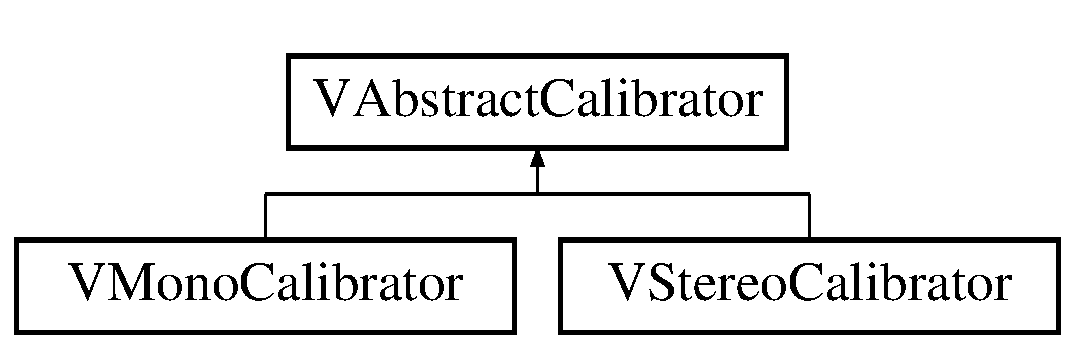
\includegraphics[height=2cm]{classVAbstractCalibrator}
\end{center}
\end{figure}
\subsection*{Public Member Functions}
\begin{DoxyCompactItemize}
\item 
\hypertarget{classVAbstractCalibrator_a7df2c56a5879435491b0153fcd5f6a6a}{
void \hyperlink{classVAbstractCalibrator_a7df2c56a5879435491b0153fcd5f6a6a}{stop} ()}
\label{classVAbstractCalibrator_a7df2c56a5879435491b0153fcd5f6a6a}

\begin{DoxyCompactList}\small\item\em Stop calibration. \item\end{DoxyCompactList}\item 
int \hyperlink{classVAbstractCalibrator_a35e8e4978841f1fe517b25eee89f491e}{getRequiredFramesCount} () const 
\item 
int \hyperlink{classVAbstractCalibrator_a76dce19c461a257a803299d7f87d5e5a}{getGrabedFramesCount} () const 
\item 
void \hyperlink{classVAbstractCalibrator_ab4eabbb2a1ce73af601c5fee87da5e24}{setResolution} (const cv::Size \&resolution)
\item 
void \hyperlink{classVAbstractCalibrator_a52f0c84c3d9398102be43f4304d2fa18}{start} (double initialFocus=-\/1.0)
\item 
virtual void \hyperlink{classVAbstractCalibrator_a2c6ac60861d16f185930e7fbf09483f8}{setRequiredFramesCount} (size\_\-t count, int squareLength)
\item 
virtual bool \hyperlink{classVAbstractCalibrator_a7251a0da257534695adcec223d467835}{calibrate} ()=0
\end{DoxyCompactItemize}
\subsection*{Static Protected Member Functions}
\begin{DoxyCompactItemize}
\item 
{\footnotesize template$<$typename Point2D $>$ }\\static void \hyperlink{classVAbstractCalibrator_aa1ce901379c3c1464887a3ef89059e60}{orderDetectedPoints} (std::vector$<$ Point2D $>$ \&points)
\end{DoxyCompactItemize}
\subsection*{Protected Attributes}
\begin{DoxyCompactItemize}
\item 
\hypertarget{classVAbstractCalibrator_ae21ea1292d7c78c8bc995fb2820e2119}{
size\_\-t \hyperlink{classVAbstractCalibrator_ae21ea1292d7c78c8bc995fb2820e2119}{m\_\-framesGrabed}}
\label{classVAbstractCalibrator_ae21ea1292d7c78c8bc995fb2820e2119}

\begin{DoxyCompactList}\small\item\em Number of grabed chessboard's views. \item\end{DoxyCompactList}\item 
\hypertarget{classVAbstractCalibrator_aebea62e01958bad93f8f56eadcf96d07}{
std::vector$<$ std::vector$<$ cv::Point3f $>$ $>$ \hyperlink{classVAbstractCalibrator_aebea62e01958bad93f8f56eadcf96d07}{m\_\-realPoints}}
\label{classVAbstractCalibrator_aebea62e01958bad93f8f56eadcf96d07}

\begin{DoxyCompactList}\small\item\em Positions of chessboard's corners in the camera's coordinate system. \item\end{DoxyCompactList}\item 
\hypertarget{classVAbstractCalibrator_a236338405da6efedfa91323af74da459}{
cv::Size \hyperlink{classVAbstractCalibrator_a236338405da6efedfa91323af74da459}{m\_\-cameraResolution}}
\label{classVAbstractCalibrator_a236338405da6efedfa91323af74da459}

\begin{DoxyCompactList}\small\item\em Resolution of the calibrating camera(s). \item\end{DoxyCompactList}\item 
\hypertarget{classVAbstractCalibrator_a94f9700184fc2c69a72aa56e661be6f4}{
double {\bfseries m\_\-initialFocusValue}}
\label{classVAbstractCalibrator_a94f9700184fc2c69a72aa56e661be6f4}

\end{DoxyCompactItemize}
\subsection*{Static Protected Attributes}
\begin{DoxyCompactItemize}
\item 
\hypertarget{classVAbstractCalibrator_ab9d3983a50f6314e1702a245eea9c8d0}{
static const cv::Size \hyperlink{classVAbstractCalibrator_ab9d3983a50f6314e1702a245eea9c8d0}{patternSize}}
\label{classVAbstractCalibrator_ab9d3983a50f6314e1702a245eea9c8d0}

\begin{DoxyCompactList}\small\item\em Nubmer of squares on eachchessboard's side. \item\end{DoxyCompactList}\end{DoxyCompactItemize}


\subsection{Detailed Description}
Base class for calibrating cameras. It uses chessboard as calibration object.

\begin{DoxyAuthor}{Author}
Dmitry Suvorov 
\end{DoxyAuthor}


\subsection{Member Function Documentation}
\hypertarget{classVAbstractCalibrator_a7251a0da257534695adcec223d467835}{
\index{VAbstractCalibrator@{VAbstractCalibrator}!calibrate@{calibrate}}
\index{calibrate@{calibrate}!VAbstractCalibrator@{VAbstractCalibrator}}
\subsubsection[{calibrate}]{\setlength{\rightskip}{0pt plus 5cm}virtual bool VAbstractCalibrator::calibrate ()\hspace{0.3cm}{\ttfamily  \mbox{[}pure virtual\mbox{]}}}}
\label{classVAbstractCalibrator_a7251a0da257534695adcec223d467835}
Calculate parameters. \begin{DoxyReturn}{Returns}
True on success. 
\end{DoxyReturn}


Implemented in \hyperlink{classVMonoCalibrator_a16cdc1f9c47d6437a124bd5f5a4ec426}{VMonoCalibrator}, and \hyperlink{classVStereoCalibrator_a7754bdddf997110220fedb2a222001ee}{VStereoCalibrator}.

\hypertarget{classVAbstractCalibrator_a76dce19c461a257a803299d7f87d5e5a}{
\index{VAbstractCalibrator@{VAbstractCalibrator}!getGrabedFramesCount@{getGrabedFramesCount}}
\index{getGrabedFramesCount@{getGrabedFramesCount}!VAbstractCalibrator@{VAbstractCalibrator}}
\subsubsection[{getGrabedFramesCount}]{\setlength{\rightskip}{0pt plus 5cm}int VAbstractCalibrator::getGrabedFramesCount () const\hspace{0.3cm}{\ttfamily  \mbox{[}inline\mbox{]}}}}
\label{classVAbstractCalibrator_a76dce19c461a257a803299d7f87d5e5a}
\begin{DoxyReturn}{Returns}
Number of grabed chessboard's views. 
\end{DoxyReturn}
\hypertarget{classVAbstractCalibrator_a35e8e4978841f1fe517b25eee89f491e}{
\index{VAbstractCalibrator@{VAbstractCalibrator}!getRequiredFramesCount@{getRequiredFramesCount}}
\index{getRequiredFramesCount@{getRequiredFramesCount}!VAbstractCalibrator@{VAbstractCalibrator}}
\subsubsection[{getRequiredFramesCount}]{\setlength{\rightskip}{0pt plus 5cm}int VAbstractCalibrator::getRequiredFramesCount () const\hspace{0.3cm}{\ttfamily  \mbox{[}inline\mbox{]}}}}
\label{classVAbstractCalibrator_a35e8e4978841f1fe517b25eee89f491e}
\begin{DoxyReturn}{Returns}
Number of chessboard's views required for calibration. 
\end{DoxyReturn}
\hypertarget{classVAbstractCalibrator_aa1ce901379c3c1464887a3ef89059e60}{
\index{VAbstractCalibrator@{VAbstractCalibrator}!orderDetectedPoints@{orderDetectedPoints}}
\index{orderDetectedPoints@{orderDetectedPoints}!VAbstractCalibrator@{VAbstractCalibrator}}
\subsubsection[{orderDetectedPoints}]{\setlength{\rightskip}{0pt plus 5cm}template$<$typename Point2D $>$ void VAbstractCalibrator::orderDetectedPoints (std::vector$<$ Point2D $>$ \& {\em points})\hspace{0.3cm}{\ttfamily  \mbox{[}inline, static, protected\mbox{]}}}}
\label{classVAbstractCalibrator_aa1ce901379c3c1464887a3ef89059e60}

\begin{DoxyParams}{Parameters}
\item[\mbox{$\leftarrow$} {\em points}]Detected chessboard's corners. \end{DoxyParams}
\hypertarget{classVAbstractCalibrator_a2c6ac60861d16f185930e7fbf09483f8}{
\index{VAbstractCalibrator@{VAbstractCalibrator}!setRequiredFramesCount@{setRequiredFramesCount}}
\index{setRequiredFramesCount@{setRequiredFramesCount}!VAbstractCalibrator@{VAbstractCalibrator}}
\subsubsection[{setRequiredFramesCount}]{\setlength{\rightskip}{0pt plus 5cm}void VAbstractCalibrator::setRequiredFramesCount (size\_\-t {\em count}, \/  int {\em squareLength})\hspace{0.3cm}{\ttfamily  \mbox{[}virtual\mbox{]}}}}
\label{classVAbstractCalibrator_a2c6ac60861d16f185930e7fbf09483f8}
Set number of chessboard's views required for calibration. param\mbox{[}in\mbox{]} count Number of chessboard's views required for calibration. param\mbox{[}in\mbox{]} squareLength Length in mm of one chessboard's square. 

Reimplemented in \hyperlink{classVMonoCalibrator_ab3b2f7b28e77094385046d9eb53569ce}{VMonoCalibrator}, and \hyperlink{classVStereoCalibrator_a48004bae492ead13c14f0810b74bc4d0}{VStereoCalibrator}.

\hypertarget{classVAbstractCalibrator_ab4eabbb2a1ce73af601c5fee87da5e24}{
\index{VAbstractCalibrator@{VAbstractCalibrator}!setResolution@{setResolution}}
\index{setResolution@{setResolution}!VAbstractCalibrator@{VAbstractCalibrator}}
\subsubsection[{setResolution}]{\setlength{\rightskip}{0pt plus 5cm}void VAbstractCalibrator::setResolution (const cv::Size \& {\em resolution})\hspace{0.3cm}{\ttfamily  \mbox{[}inline\mbox{]}}}}
\label{classVAbstractCalibrator_ab4eabbb2a1ce73af601c5fee87da5e24}
Set camera's resolution. 
\begin{DoxyParams}{Parameters}
\item[\mbox{$\leftarrow$} {\em resolution}]Resolution of the calibrating camera(s). \end{DoxyParams}
\hypertarget{classVAbstractCalibrator_a52f0c84c3d9398102be43f4304d2fa18}{
\index{VAbstractCalibrator@{VAbstractCalibrator}!start@{start}}
\index{start@{start}!VAbstractCalibrator@{VAbstractCalibrator}}
\subsubsection[{start}]{\setlength{\rightskip}{0pt plus 5cm}void VAbstractCalibrator::start (double {\em initialFocus} = {\ttfamily -\/1.0})\hspace{0.3cm}{\ttfamily  \mbox{[}inline\mbox{]}}}}
\label{classVAbstractCalibrator_a52f0c84c3d9398102be43f4304d2fa18}
Start calibration. 
\begin{DoxyParams}{Parameters}
\item[\mbox{$\leftarrow$} {\em initialFocus}]Initial focus value in pixels. \end{DoxyParams}


The documentation for this class was generated from the following files:\begin{DoxyCompactItemize}
\item 
\hyperlink{v__abstract__calibrator_8h}{v\_\-abstract\_\-calibrator.h}\item 
v\_\-abstract\_\-calibrator.cpp\end{DoxyCompactItemize}

\hypertarget{classVMonoCalibrator}{
\section{VMonoCalibrator Class Reference}
\label{classVMonoCalibrator}\index{VMonoCalibrator@{VMonoCalibrator}}
}


{\ttfamily \#include $<$v\_\-mono\_\-calibrator.h$>$}

Inheritance diagram for VMonoCalibrator:\begin{figure}[H]
\begin{center}
\leavevmode
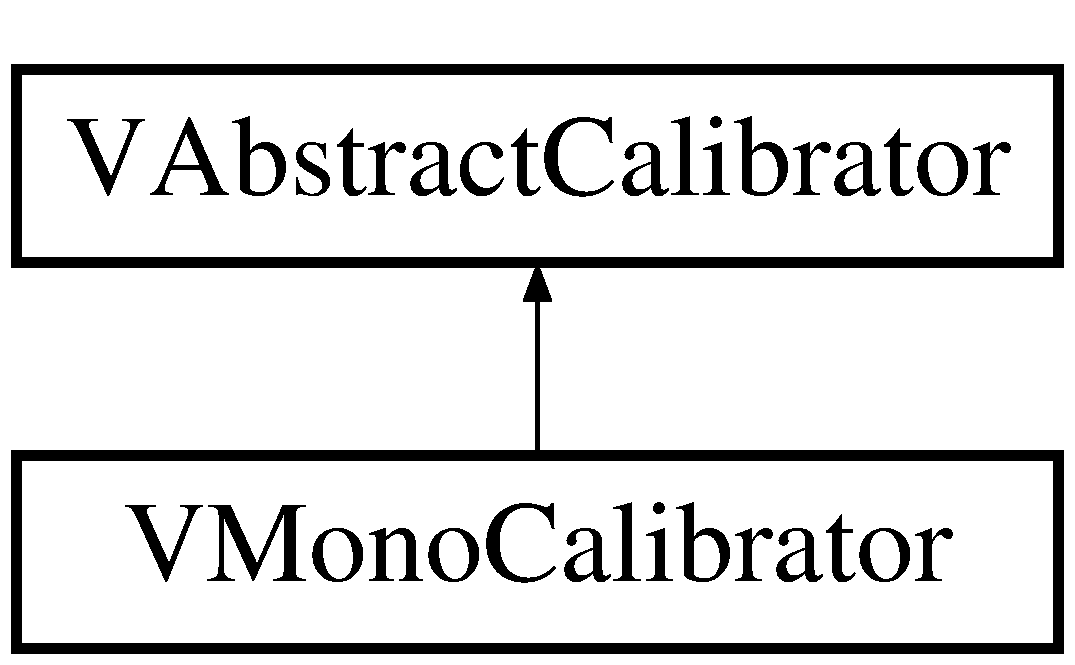
\includegraphics[height=2cm]{classVMonoCalibrator}
\end{center}
\end{figure}
\subsection*{Public Member Functions}
\begin{DoxyCompactItemize}
\item 
int \hyperlink{classVMonoCalibrator_a026938d74f2c8c2c6df06f8e50270b16}{tryFrame} (cv::Mat \&frame)
\item 
void \hyperlink{classVMonoCalibrator_a041c63fcebcf35b1277027c0d18a7d47}{getHomography} (cv::Mat \&H) const 
\item 
void \hyperlink{classVMonoCalibrator_a0acebdd3d00dcf56a5bbb119f6572ba8}{getIntrinsics} (cv::Mat \&M, cv::Mat \&D) const 
\item 
void \hyperlink{classVMonoCalibrator_a1a3aa1b57538d2bfd993ecf8c0b2e4fd}{getExtrinsics} (cv::Mat \&R, cv::Mat \&T) const 
\item 
virtual void \hyperlink{classVMonoCalibrator_ab3b2f7b28e77094385046d9eb53569ce}{setRequiredFramesCount} (size\_\-t count, int squareLength)
\item 
virtual bool \hyperlink{classVMonoCalibrator_a16cdc1f9c47d6437a124bd5f5a4ec426}{calibrate} ()
\end{DoxyCompactItemize}


\subsection{Detailed Description}
Class for calibrating one camera using chessboard.

\begin{DoxyAuthor}{Author}
Dmitry Suvorov 
\end{DoxyAuthor}


\subsection{Member Function Documentation}
\hypertarget{classVMonoCalibrator_a16cdc1f9c47d6437a124bd5f5a4ec426}{
\index{VMonoCalibrator@{VMonoCalibrator}!calibrate@{calibrate}}
\index{calibrate@{calibrate}!VMonoCalibrator@{VMonoCalibrator}}
\subsubsection[{calibrate}]{\setlength{\rightskip}{0pt plus 5cm}bool VMonoCalibrator::calibrate ()\hspace{0.3cm}{\ttfamily  \mbox{[}virtual\mbox{]}}}}
\label{classVMonoCalibrator_a16cdc1f9c47d6437a124bd5f5a4ec426}
Calculate parameters. \begin{DoxyReturn}{Returns}
True on success. 
\end{DoxyReturn}


Implements \hyperlink{classVAbstractCalibrator_a7251a0da257534695adcec223d467835}{VAbstractCalibrator}.

\hypertarget{classVMonoCalibrator_a1a3aa1b57538d2bfd993ecf8c0b2e4fd}{
\index{VMonoCalibrator@{VMonoCalibrator}!getExtrinsics@{getExtrinsics}}
\index{getExtrinsics@{getExtrinsics}!VMonoCalibrator@{VMonoCalibrator}}
\subsubsection[{getExtrinsics}]{\setlength{\rightskip}{0pt plus 5cm}void VMonoCalibrator::getExtrinsics (cv::Mat \& {\em R}, \/  cv::Mat \& {\em T}) const\hspace{0.3cm}{\ttfamily  \mbox{[}inline\mbox{]}}}}
\label{classVMonoCalibrator_a1a3aa1b57538d2bfd993ecf8c0b2e4fd}
Get extrinsics camera's parameters. 
\begin{DoxyParams}{Parameters}
\item[\mbox{$\rightarrow$} {\em R}]Rotation vector. \item[\mbox{$\rightarrow$} {\em T}]Translation vector. \end{DoxyParams}
\hypertarget{classVMonoCalibrator_a041c63fcebcf35b1277027c0d18a7d47}{
\index{VMonoCalibrator@{VMonoCalibrator}!getHomography@{getHomography}}
\index{getHomography@{getHomography}!VMonoCalibrator@{VMonoCalibrator}}
\subsubsection[{getHomography}]{\setlength{\rightskip}{0pt plus 5cm}void VMonoCalibrator::getHomography (cv::Mat \& {\em H}) const}}
\label{classVMonoCalibrator_a041c63fcebcf35b1277027c0d18a7d47}
Get Homography(transformation matrix from camera's coordinates to image coordinates). 
\begin{DoxyParams}{Parameters}
\item[\mbox{$\rightarrow$} {\em H}]Matrix 4x3. \end{DoxyParams}
\hypertarget{classVMonoCalibrator_a0acebdd3d00dcf56a5bbb119f6572ba8}{
\index{VMonoCalibrator@{VMonoCalibrator}!getIntrinsics@{getIntrinsics}}
\index{getIntrinsics@{getIntrinsics}!VMonoCalibrator@{VMonoCalibrator}}
\subsubsection[{getIntrinsics}]{\setlength{\rightskip}{0pt plus 5cm}void VMonoCalibrator::getIntrinsics (cv::Mat \& {\em M}, \/  cv::Mat \& {\em D}) const\hspace{0.3cm}{\ttfamily  \mbox{[}inline\mbox{]}}}}
\label{classVMonoCalibrator_a0acebdd3d00dcf56a5bbb119f6572ba8}
Get intisics camera's parameters. 
\begin{DoxyParams}{Parameters}
\item[\mbox{$\rightarrow$} {\em M}]Camera's matrix. \item[\mbox{$\rightarrow$} {\em D}]Distortion coefficients. \end{DoxyParams}
\hypertarget{classVMonoCalibrator_ab3b2f7b28e77094385046d9eb53569ce}{
\index{VMonoCalibrator@{VMonoCalibrator}!setRequiredFramesCount@{setRequiredFramesCount}}
\index{setRequiredFramesCount@{setRequiredFramesCount}!VMonoCalibrator@{VMonoCalibrator}}
\subsubsection[{setRequiredFramesCount}]{\setlength{\rightskip}{0pt plus 5cm}void VMonoCalibrator::setRequiredFramesCount (size\_\-t {\em count}, \/  int {\em squareLength})\hspace{0.3cm}{\ttfamily  \mbox{[}virtual\mbox{]}}}}
\label{classVMonoCalibrator_ab3b2f7b28e77094385046d9eb53569ce}
Set number of chessboard's views required for calibration. param\mbox{[}in\mbox{]} count Number of chessboard's views required for calibration. param\mbox{[}in\mbox{]} squareLength Length in mm of one chessboard's square. 

Reimplemented from \hyperlink{classVAbstractCalibrator_a2c6ac60861d16f185930e7fbf09483f8}{VAbstractCalibrator}.

\hypertarget{classVMonoCalibrator_a026938d74f2c8c2c6df06f8e50270b16}{
\index{VMonoCalibrator@{VMonoCalibrator}!tryFrame@{tryFrame}}
\index{tryFrame@{tryFrame}!VMonoCalibrator@{VMonoCalibrator}}
\subsubsection[{tryFrame}]{\setlength{\rightskip}{0pt plus 5cm}int VMonoCalibrator::tryFrame (cv::Mat \& {\em frame})}}
\label{classVMonoCalibrator_a026938d74f2c8c2c6df06f8e50270b16}
Try to detect chessboard's corners. 
\begin{DoxyParams}{Parameters}
\item[\mbox{$\leftarrow$} {\em frame}]Image with chessboard. \end{DoxyParams}
\begin{DoxyReturn}{Returns}
Number of frames to grab before starting calibration. 
\end{DoxyReturn}


The documentation for this class was generated from the following files:\begin{DoxyCompactItemize}
\item 
\hyperlink{v__mono__calibrator_8h}{v\_\-mono\_\-calibrator.h}\item 
v\_\-mono\_\-calibrator.cpp\end{DoxyCompactItemize}

\hypertarget{classVStereoCalibrator}{
\section{VStereoCalibrator Class Reference}
\label{classVStereoCalibrator}\index{VStereoCalibrator@{VStereoCalibrator}}
}


{\ttfamily \#include $<$v\_\-stereo\_\-calibrator.h$>$}

Inheritance diagram for VStereoCalibrator:\begin{figure}[H]
\begin{center}
\leavevmode
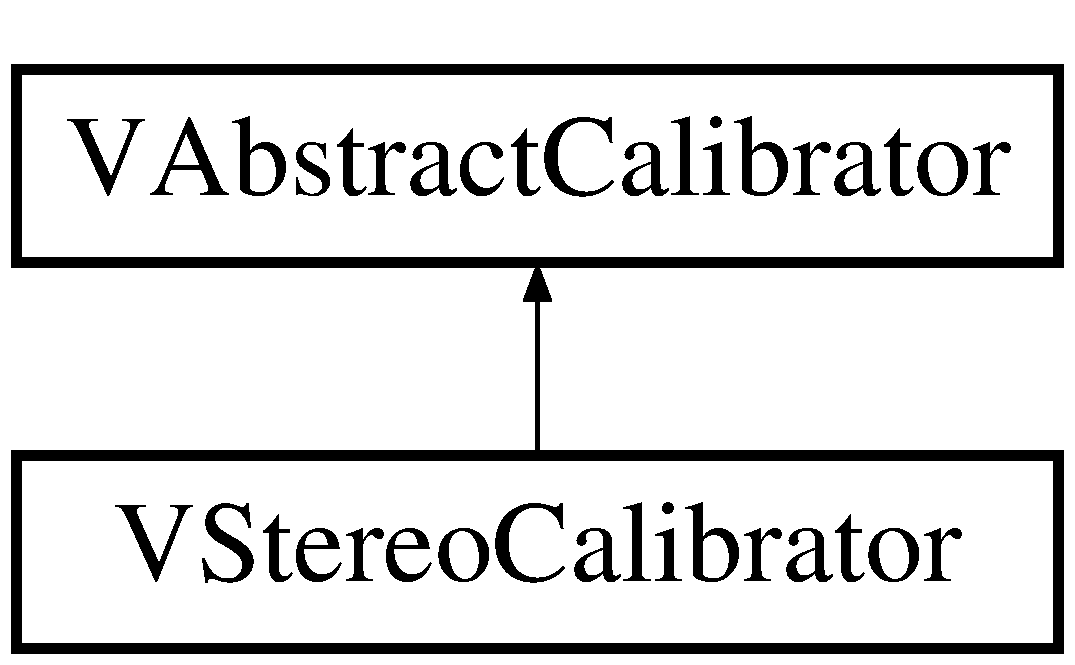
\includegraphics[height=2cm]{classVStereoCalibrator}
\end{center}
\end{figure}
\subsection*{Public Types}
\begin{DoxyCompactItemize}
\item 
enum \hyperlink{classVStereoCalibrator_a2a31c8af7740705eda798588a5311fb7}{CameraSide} \{ {\bfseries LEFT\_\-CAMERA}, 
{\bfseries RIGHT\_\-CAMERA}
 \}
\begin{DoxyCompactList}\small\item\em Camera's position in the stereo system. \item\end{DoxyCompactList}\item 
enum \{ {\bfseries CAMERAS\_\-COUNT} =  2
 \}
\begin{DoxyCompactList}\small\item\em Count of cameras in the stereo system. \item\end{DoxyCompactList}\end{DoxyCompactItemize}
\subsection*{Public Member Functions}
\begin{DoxyCompactItemize}
\item 
\hypertarget{classVStereoCalibrator_a99cf01815e1a586f39f3da5d8d37848f}{
void \hyperlink{classVStereoCalibrator_a99cf01815e1a586f39f3da5d8d37848f}{getCamerasIntrinsics} (int side, cv::Mat \&M, cv::Mat \&D) const }
\label{classVStereoCalibrator_a99cf01815e1a586f39f3da5d8d37848f}

\begin{DoxyCompactList}\small\item\em Get intrinsics parameters of one camera. \item\end{DoxyCompactList}\item 
\hypertarget{classVStereoCalibrator_a00919cac74070cd925bfe8e05046a44a}{
void \hyperlink{classVStereoCalibrator_a00919cac74070cd925bfe8e05046a44a}{getEssentialMatrix} (cv::Mat \&E) const }
\label{classVStereoCalibrator_a00919cac74070cd925bfe8e05046a44a}

\begin{DoxyCompactList}\small\item\em Get essential matrix. \item\end{DoxyCompactList}\item 
\hypertarget{classVStereoCalibrator_aebd902a53410b7a9a4df570fcd5245c0}{
void \hyperlink{classVStereoCalibrator_aebd902a53410b7a9a4df570fcd5245c0}{getFundamentalMatrix} (cv::Mat \&F) const }
\label{classVStereoCalibrator_aebd902a53410b7a9a4df570fcd5245c0}

\begin{DoxyCompactList}\small\item\em Get fundamental matrix. \item\end{DoxyCompactList}\item 
\hypertarget{classVStereoCalibrator_a4d61328f70d43a5414f5e9a53ffd642b}{
void \hyperlink{classVStereoCalibrator_a4d61328f70d43a5414f5e9a53ffd642b}{getCamerasOrientation} (cv::Mat \&R, cv::Mat \&T) const }
\label{classVStereoCalibrator_a4d61328f70d43a5414f5e9a53ffd642b}

\begin{DoxyCompactList}\small\item\em Get the rotation matrix and translation vector between the cameras. \item\end{DoxyCompactList}\item 
int \hyperlink{classVStereoCalibrator_ac080bd54496fef9b9e115944ddc3ca34}{tryFrames} (cv::Mat \&leftFrame, cv::Mat \&rightFrame)
\item 
virtual void \hyperlink{classVStereoCalibrator_a48004bae492ead13c14f0810b74bc4d0}{setRequiredFramesCount} (size\_\-t count, int squareLength)
\item 
virtual bool \hyperlink{classVStereoCalibrator_a7754bdddf997110220fedb2a222001ee}{calibrate} ()
\end{DoxyCompactItemize}


\subsection{Detailed Description}
Class for calibrating stereo system using chessboard.

\begin{DoxyAuthor}{Author}
Dmitry Suvorov 
\end{DoxyAuthor}


\subsection{Member Function Documentation}
\hypertarget{classVStereoCalibrator_a7754bdddf997110220fedb2a222001ee}{
\index{VStereoCalibrator@{VStereoCalibrator}!calibrate@{calibrate}}
\index{calibrate@{calibrate}!VStereoCalibrator@{VStereoCalibrator}}
\subsubsection[{calibrate}]{\setlength{\rightskip}{0pt plus 5cm}bool VStereoCalibrator::calibrate ()\hspace{0.3cm}{\ttfamily  \mbox{[}virtual\mbox{]}}}}
\label{classVStereoCalibrator_a7754bdddf997110220fedb2a222001ee}
Calculate parameters. \begin{DoxyReturn}{Returns}
True on success. 
\end{DoxyReturn}


Implements \hyperlink{classVAbstractCalibrator_a7251a0da257534695adcec223d467835}{VAbstractCalibrator}.

\hypertarget{classVStereoCalibrator_a48004bae492ead13c14f0810b74bc4d0}{
\index{VStereoCalibrator@{VStereoCalibrator}!setRequiredFramesCount@{setRequiredFramesCount}}
\index{setRequiredFramesCount@{setRequiredFramesCount}!VStereoCalibrator@{VStereoCalibrator}}
\subsubsection[{setRequiredFramesCount}]{\setlength{\rightskip}{0pt plus 5cm}void VStereoCalibrator::setRequiredFramesCount (size\_\-t {\em count}, \/  int {\em squareLength})\hspace{0.3cm}{\ttfamily  \mbox{[}virtual\mbox{]}}}}
\label{classVStereoCalibrator_a48004bae492ead13c14f0810b74bc4d0}
Set number of chessboard's views required for calibration. param\mbox{[}in\mbox{]} count Number of chessboard's views required for calibration. param\mbox{[}in\mbox{]} squareLength Length in mm of one chessboard's square. 

Reimplemented from \hyperlink{classVAbstractCalibrator_a2c6ac60861d16f185930e7fbf09483f8}{VAbstractCalibrator}.

\hypertarget{classVStereoCalibrator_ac080bd54496fef9b9e115944ddc3ca34}{
\index{VStereoCalibrator@{VStereoCalibrator}!tryFrames@{tryFrames}}
\index{tryFrames@{tryFrames}!VStereoCalibrator@{VStereoCalibrator}}
\subsubsection[{tryFrames}]{\setlength{\rightskip}{0pt plus 5cm}int VStereoCalibrator::tryFrames (cv::Mat \& {\em leftFrame}, \/  cv::Mat \& {\em rightFrame})}}
\label{classVStereoCalibrator_ac080bd54496fef9b9e115944ddc3ca34}
Try to detect chessboard's corners. 
\begin{DoxyParams}{Parameters}
\item[\mbox{$\leftarrow$} {\em frame}]Image with chessboard. \end{DoxyParams}
\begin{DoxyReturn}{Returns}
Number of frames to grab before starting calibration. 
\end{DoxyReturn}


The documentation for this class was generated from the following files:\begin{DoxyCompactItemize}
\item 
\hyperlink{v__stereo__calibrator_8h}{v\_\-stereo\_\-calibrator.h}\item 
v\_\-stereo\_\-calibrator.cpp\end{DoxyCompactItemize}

\chapter{File Documentation}
\hypertarget{v__abstract__calibrator_8h}{
\section{v\_\-abstract\_\-calibrator.h File Reference}
\label{v__abstract__calibrator_8h}\index{v\_\-abstract\_\-calibrator.h@{v\_\-abstract\_\-calibrator.h}}
}


Definition of the base class for calibration.  


{\ttfamily \#include $<$opencv2/core/core.hpp$>$}\par
\subsection*{Classes}
\begin{DoxyCompactItemize}
\item 
class \hyperlink{classVAbstractCalibrator}{VAbstractCalibrator}
\end{DoxyCompactItemize}


\subsection{Detailed Description}
Definition of the base class for calibration. This program is free software; you can redistribute it and/or modify it under the terms of the GNU General Public License as published by the Free Software Foundation; either version 2 of the License, or (at your option) any later version.

This program is distributed in the hope that it will be useful, but WITHOUT ANY WARRANTY; without even the implied warranty of MERCHANTABILITY or FITNESS FOR A PARTICULAR PURPOSE. See the GNU General Public License for more details.

You should have received a copy of the GNU General Public License along with this program; if not, write to the Free Software Foundation, Inc., 51 Franklin Street, Fifth Floor, Boston, MA 02110-\/1301, USA. 
\hypertarget{v__mono__calibrator_8h}{
\section{v\_\-mono\_\-calibrator.h File Reference}
\label{v__mono__calibrator_8h}\index{v\_\-mono\_\-calibrator.h@{v\_\-mono\_\-calibrator.h}}
}


Definition of the class for calibration one camera.  


{\ttfamily \#include $<$opencv2/calib3d/calib3d.hpp$>$}\par
{\ttfamily \#include $<$opencv2/imgproc/imgproc.hpp$>$}\par
{\ttfamily \#include \char`\"{}v\_\-abstract\_\-calibrator.h\char`\"{}}\par
\subsection*{Classes}
\begin{DoxyCompactItemize}
\item 
class \hyperlink{classVMonoCalibrator}{VMonoCalibrator}
\end{DoxyCompactItemize}


\subsection{Detailed Description}
Definition of the class for calibration one camera. This program is free software; you can redistribute it and/or modify it under the terms of the GNU General Public License as published by the Free Software Foundation; either version 2 of the License, or (at your option) any later version.

This program is distributed in the hope that it will be useful, but WITHOUT ANY WARRANTY; without even the implied warranty of MERCHANTABILITY or FITNESS FOR A PARTICULAR PURPOSE. See the GNU General Public License for more details.

You should have received a copy of the GNU General Public License along with this program; if not, write to the Free Software Foundation, Inc., 51 Franklin Street, Fifth Floor, Boston, MA 02110-\/1301, USA. 
\hypertarget{v__stereo__calibrator_8h}{
\section{v\_\-stereo\_\-calibrator.h File Reference}
\label{v__stereo__calibrator_8h}\index{v\_\-stereo\_\-calibrator.h@{v\_\-stereo\_\-calibrator.h}}
}


Definition of class for calibrating stereo system.  


{\ttfamily \#include $<$opencv2/calib3d/calib3d.hpp$>$}\par
{\ttfamily \#include \char`\"{}v\_\-abstract\_\-calibrator.h\char`\"{}}\par
\subsection*{Classes}
\begin{DoxyCompactItemize}
\item 
class \hyperlink{classVStereoCalibrator}{VStereoCalibrator}
\end{DoxyCompactItemize}


\subsection{Detailed Description}
Definition of class for calibrating stereo system. This program is free software; you can redistribute it and/or modify it under the terms of the GNU General Public License as published by the Free Software Foundation; either version 2 of the License, or (at your option) any later version.

This program is distributed in the hope that it will be useful, but WITHOUT ANY WARRANTY; without even the implied warranty of MERCHANTABILITY or FITNESS FOR A PARTICULAR PURPOSE. See the GNU General Public License for more details.

You should have received a copy of the GNU General Public License along with this program; if not, write to the Free Software Foundation, Inc., 51 Franklin Street, Fifth Floor, Boston, MA 02110-\/1301, USA. 
\printindex
\end{document}
